\documentclass[10pt]{beamer}
\usetheme{Malmoe}
\colorlet{beamer@blendedblue}{green!40!black}
\setbeamertemplate{navigation symbols}{}
\newcommand*\oldmacro{}%
\let\oldmacro\insertshorttitle%
\renewcommand*\insertshorttitle{%
\oldmacro\hfill%
\insertframenumber\,/\,\inserttotalframenumber}

\usepackage{caption}
\usepackage{hyperref}
\usepackage[makeroom]{cancel}
\usepackage{ amssymb }
\usepackage{appendixnumberbeamer}
%\usepackage{tikz-feynman}
\usepackage{graphicx}
\begin{document}
\title{Search for Flavor Changing Neutral Currents in Top Quark Decays}
\subtitle{$t \rightarrow q \gamma$}
\subtitle{B-Tagging Working Point and $e \rightarrow \gamma$ Fakes}
\author[Barkeloo]{Jason Barkeloo}

\titlegraphic{
\includegraphics[width=4cm]{../ATLAS-Logo-Ref-RGB.png}\hspace*{2.75cm}~%
   
\includegraphics[width=4cm]{../uo_logo_green_on_white_2.jpg}
}

%\frame{\frametitle{}
%\begin{itemize}
%\item
%\end{itemize}
%}


\date{September 12, 2019}
\frame{\titlepage}
\frame{\frametitle{Overview}\tableofcontents[]}%hidesubsections]}
\section{Brief Background}
%\frame{\frametitle{Table of Contents}\tableofcontents[currentsection,hideothersubsections]}
%%%%%%%%%%%%%%%%%%%%%%%%%%%%%%%%%%%%%%%%%%%%%%%%%%%%%%%%%

\subsection{The Top Quark}

\frame{\frametitle{Top Quark Decays in the SM}
\centering
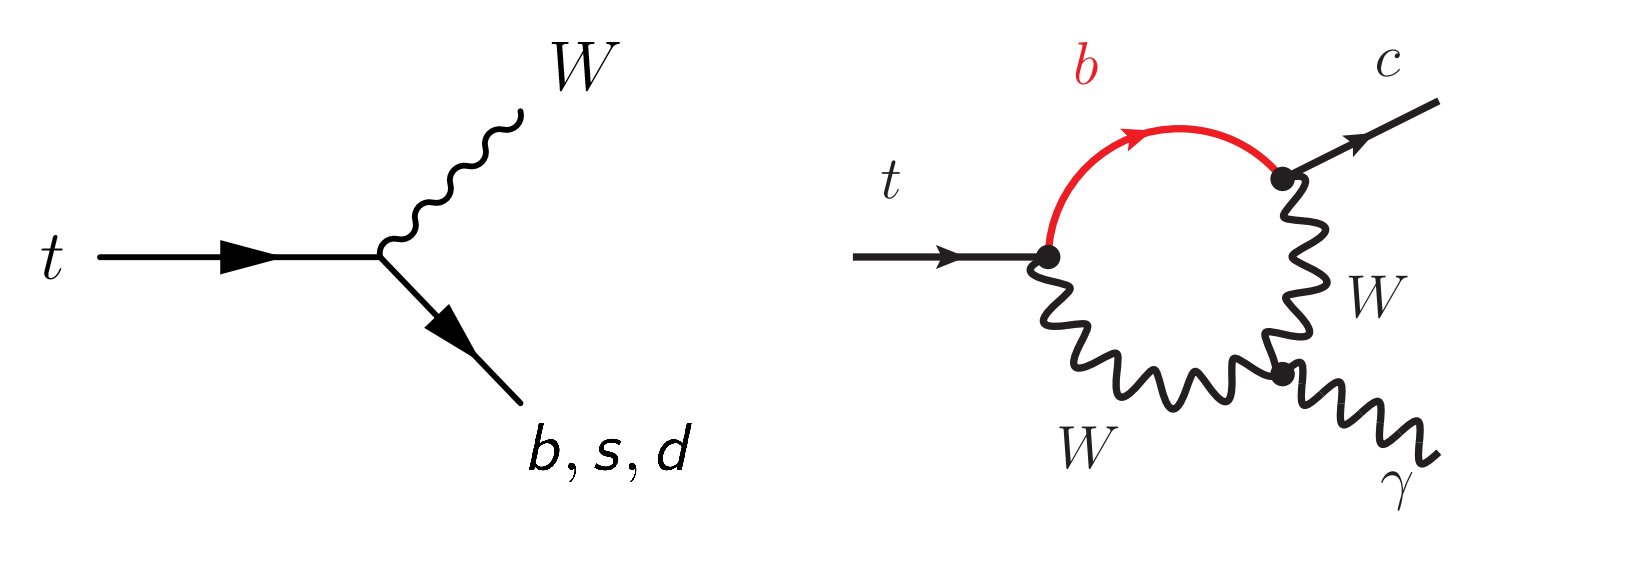
\includegraphics[width=1.\textwidth]{../../Thesis/ThesisImages/Theory/SMTopDecays2.png}

\begin{columns}
\begin{column}{0.5\textwidth}
\begin{itemize}
\item $t\rightarrow b W \approx 99.83\%$
\item $t\rightarrow s W \approx 0.16\%$
\item $t\rightarrow d W \approx 0.01\%$
\end{itemize}
\end{column}
\begin{column}{0.5\textwidth}
\begin{itemize}
\item $t\rightarrow q_{u,c} X\approx 10^{-17} - 10^{-12}$
\item Limits on $t\rightarrow \gamma q$ processes: \href{https://arxiv.org/abs/1511.03951}{[JHEP 04 (2016) 035]}
	\begin{itemize}
	\item $t\rightarrow \gamma u < 1.3 x10^{-4}$
	\item $t\rightarrow \gamma c < 1.7 x 10^{-3}$
	\end{itemize}
\end{itemize}
\end{column}
\end{columns}
}



\subsection{FCNC at the LHC} 

\frame{\frametitle{FCNC: What are we looking for? $t\bar{t}\rightarrow W (\rightarrow l \nu) b+ q\gamma$}
Will further investigate BJets here.
\begin{itemize}
\item Final state topology
	\begin{itemize}
	\item One Neutrino, from W
	\item One Lepton, from W
	\item One B-jet, SM Top
	\item One Photon, FCNC Top
	\item One Jet, FCNC Top
	\end{itemize}
\end{itemize}
\centering
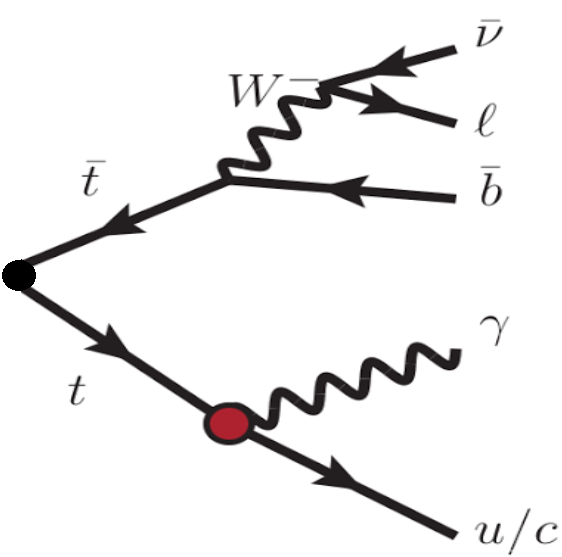
\includegraphics[width=0.35\textwidth]{../../Thesis/ThesisImages/fcncttbar.png}
}

%%%%%%%%%%%%%%%%%%%%%%%%%%%%%%%%%%%%%%%%%%%%%%%%%%%%%%%%%%%%%%%%%
%
%\subsection{Object Preselection Cuts }
%\frame{\frametitle{Object Preselection}
%\begin{itemize}
%\item We preselect events with objects that look like similar to our expected topology
%\item Require:
%	\begin{itemize}
%	\item Exactly one lepton (e or $\mu$) $\geq$ 25 GeV
%	\item Exactly one good photon $\geq$ 15GeV
%	\item Missing Transverse Energy $\geq$ 30GeV
%	\item $\geq 1$ Jets
%	\end{itemize}
%\item Further exploration of the BJets will be discussed
%\end{itemize}
%}
\section{B-tagging Working Point Selection}
\subsection{B-tagging Background}
\frame{\frametitle{B-tagging}
\begin{columns}
\begin{column}{0.5\textwidth}
\begin{itemize}
\item B Hadrons travel a measureable distance before decay
\item Tracks originate from outside of interaction point (Seconday Vertex)
\item Backtracking tracks in displaced vertex gives an impact parameter
\item Decay chain MVA attempts to reconstruct decay of the jet
\item Outputs of these algorithms used in a BDT to determine if a Jet is from a b-quark
\end{itemize}
\end{column}
\begin{column}{0.5\textwidth}
\centering
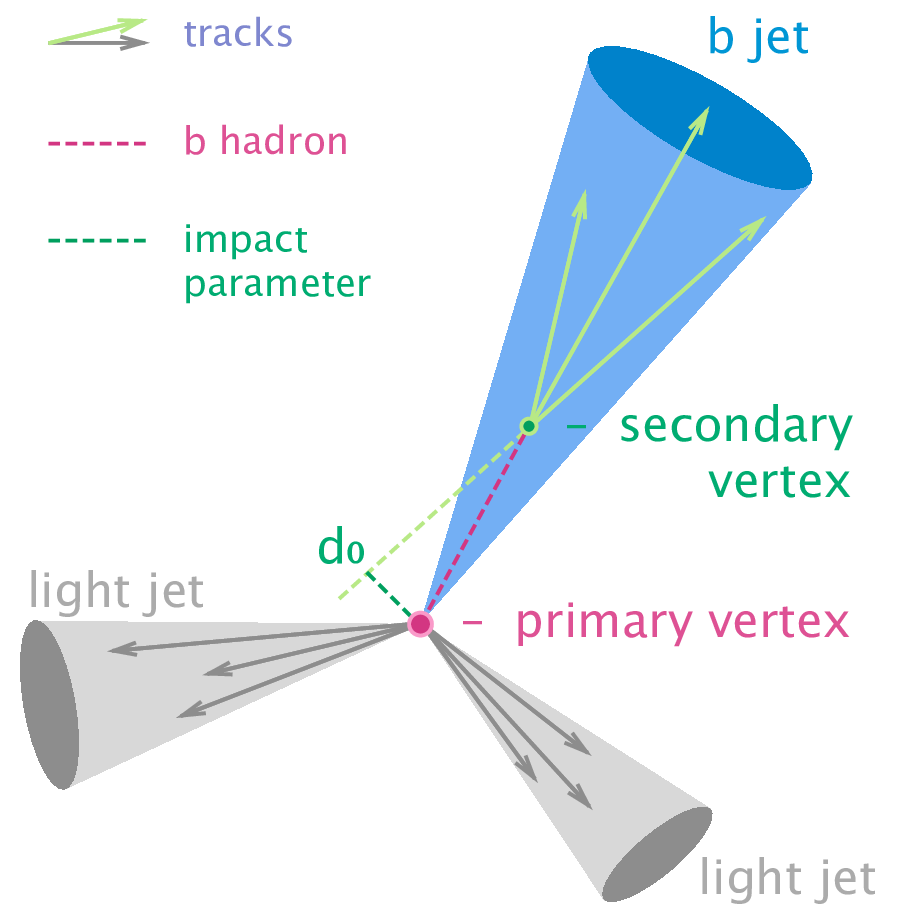
\includegraphics[height=.65\textheight]{../../Thesis/ThesisImages/SimulationNN/B-tagging_diagram.png}
\end{column}
\end{columns}
}

\frame{\frametitle{Mv2c10}
MV2c10 is used to tag b-jets. The c10 implies a 10\% c-jet fraction in the background training sample.  Can use various fixed-cut working points for b-jet identification.  \\
Using a different working point can change which jets are identified as originating from b-quarks in the analysis.
\begin{center}
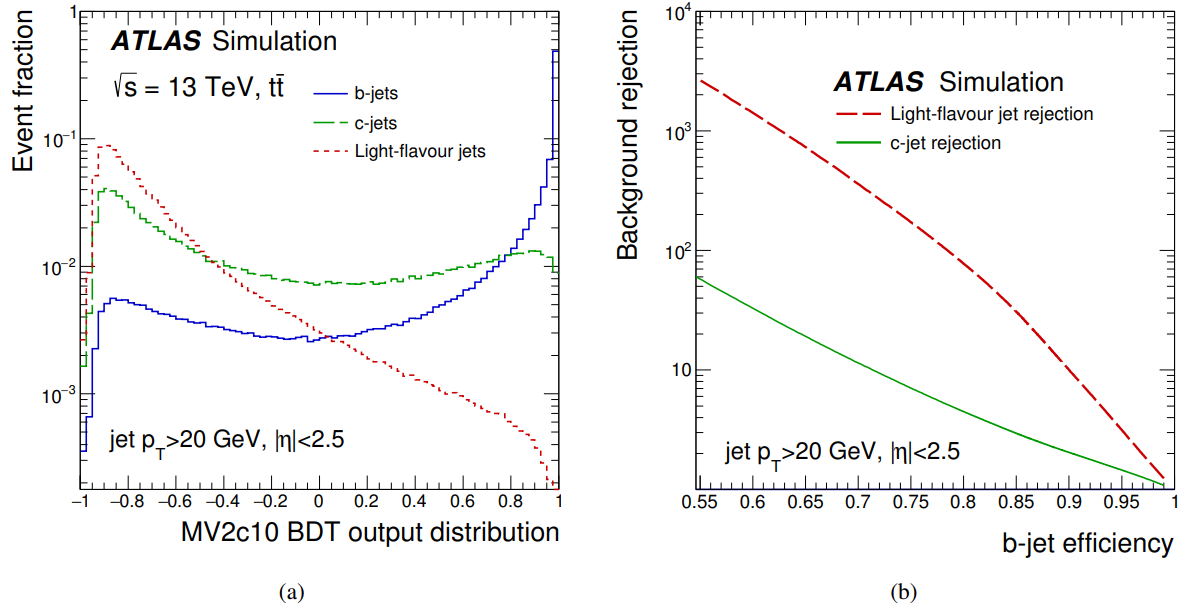
\includegraphics[width=.8\textwidth]{../../Thesis/ThesisImages/SimulationNN/BTagMV2c10andRejVsEff.png}\\
\href{https://arxiv.org/pdf/1805.01845.pdf}{JHEP 08 (2018) 89}
\end{center}
}


\subsection{Neural Network on B-tagging WPs}

\frame{\frametitle{Neural Network Reminder}
\begin{columns}
\begin{column}{0.48\textwidth}
\centering
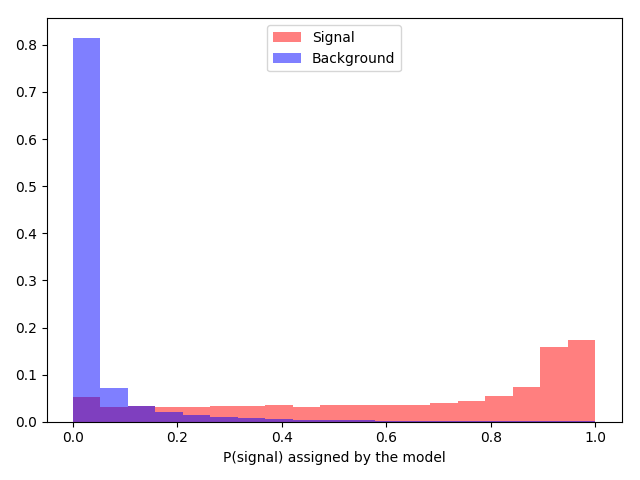
\includegraphics[width=0.85\textwidth]{Images/btag77/mujetsboth2hidnpart0sigbkg.png} 
\includegraphics[width=0.85\textwidth]{../../Thesis/ThesisImages/SimulationNN/{HiddenLayerStudiesBR0.002}/btag77/modelouts/significancemujetsboth2hidnpart02.png}
\end{column}
\begin{column}{0.48\textwidth}
\centering
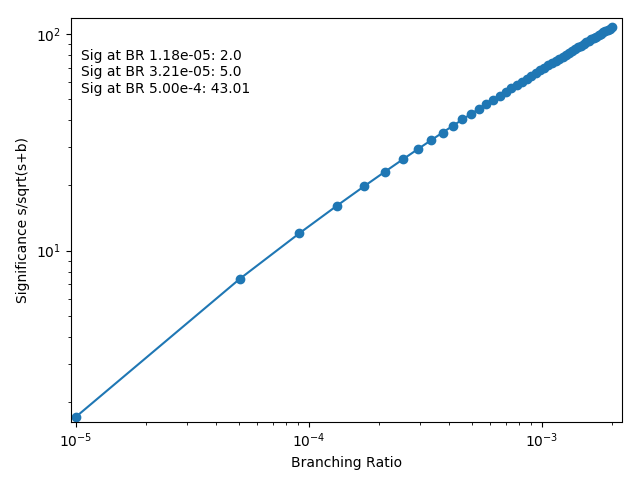
\includegraphics[width=0.85\textwidth]{Images/btag77/mujetsboth2hidnpart0SigVsBR.png} 
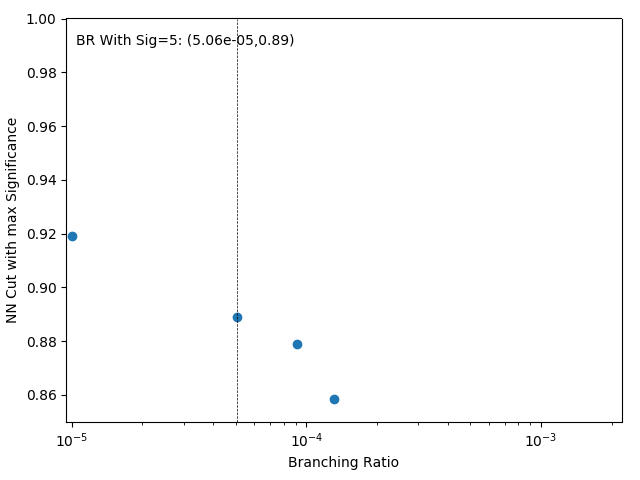
\includegraphics[width=0.85\textwidth]{Images/btag77/mujetsboth2hidnpart0CutVsBR.png} 
\end{column}
\end{columns}
Branching ratio with Significance = 2:  1.18e-5
}


\frame{\frametitle{Neural Network Results}
\begin{columns}
\begin{column}{0.02\textwidth}
\rotatebox{90}{Muon Channel \qquad  Electron Channel} 
%\rotatebox{90}{Muon Channel        } 
\end{column}
\begin{column}{0.33\textwidth}
\begin{itemize}
\item  70\% Working Point
\end{itemize}
\includegraphics[width=.95\textwidth]{../../Thesis/ThesisImages/SimulationNN/{HiddenLayerStudiesBR0.002}/btag70/modelouts/significanceejetsboth2hidnpart02.png} \\
\tiny BR with Sig=2: $1.25\times10^{-5}$\\
\includegraphics[width=.95\textwidth]{../../Thesis/ThesisImages/SimulationNN/{HiddenLayerStudiesBR0.002}/btag70/modelouts/significancemujetsboth2hidnpart02.png}\\
BR with Sig=2: $1.31\times10^{-5}$
\end{column}
\begin{column}{0.33\textwidth}
\begin{itemize}
\item 77\% Working Point
\end{itemize}
\includegraphics[width=.95\textwidth]{../../Thesis/ThesisImages/SimulationNN/{HiddenLayerStudiesBR0.002}/btag77/modelouts/significanceejetsboth2hidnpart02.png} \\
\tiny BR with Sig=2: $1.23\times10^{-5}$\\
\includegraphics[width=.95\textwidth]{../../Thesis/ThesisImages/SimulationNN/{HiddenLayerStudiesBR0.002}/btag77/modelouts/significancemujetsboth2hidnpart02.png}\\
BR with Sig=2: $1.18\times10^{-5}$
\end{column}
\begin{column}{0.33\textwidth}
\begin{itemize}
\item 85\% Working Point
\end{itemize}
\includegraphics[width=.95\textwidth]{../../Thesis/ThesisImages/SimulationNN/{HiddenLayerStudiesBR0.002}/btag85/modelouts/significanceejetsboth2hidnpart02.png} \\
\tiny BR with Sig=2: $1.28\times10^{-5}$\\
\includegraphics[width=.95\textwidth]{../../Thesis/ThesisImages/SimulationNN/{HiddenLayerStudiesBR0.002}/btag85/modelouts/significancemujetsboth2hidnpart02.png}\\
BR with Sig=2: $1.19\times10^{-5}$
\end{column}
\end{columns}
}

%\frame{\frametitle{Preselection Objects with $N_{BJet}= 1$ }
%\begin{columns}
%\begin{column}{0.02\textwidth}
%\rotatebox{90}{Muon Channel \qquad  Electron Channel} 
%%\rotatebox{90}{Muon Channel        } 
%\end{column}
%\begin{column}{0.5\textwidth}
%\begin{itemize}
%\item $\gamma_{iso}$
%\end{itemize}
%\includegraphics[width=.95\textwidth]{Images/ejetsvarplots/photon0_iso.png} \\
%\includegraphics[width=.95\textwidth]{Images/mujetsvarplots/photon0_iso.png}
%\end{column}
%\begin{column}{0.5\textwidth}
%\begin{itemize}
%\item $\Delta R_{j\gamma}$
%\end{itemize}
%\includegraphics[width=.95\textwidth]{Images/ejetsvarplots/deltaRjgam.png} \\
%\includegraphics[width=.95\textwidth]{Images/mujetsvarplots/deltaRjgam.png}
%\end{column}
%\end{columns}
%}


%%%%%%%%%%%%%%%%
\section{$e\rightarrow \gamma$ Fake Rate: Initial Studies}
\subsection{Initial Studies}

\frame{\frametitle{Fake Rate Studies}
\begin{centering}
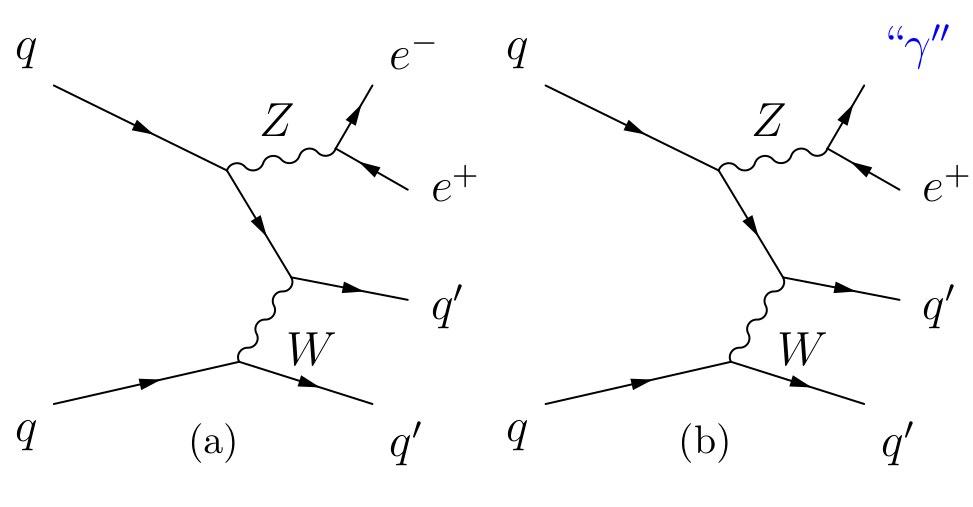
\includegraphics[width=.8\textwidth]{../../Thesis/ThesisImages/ZeeFakeDiagram.png}\\
\end{centering}
Want to be able to correct the number of fake photons predicted in MC to those present in Data
}


\frame{\frametitle{Fake Rate Object Selection}
\begin{itemize}
\item Want to calculate fake rate in events which could enter the signal region.
\item Create 2 control regions: $Z\rightarrow ee$ and $Z\rightarrow e \gamma$
\item Require:
	\begin{itemize}
	\item Common Object Selection (MET,Jets,Triggers, etc.)
	\item Exactly 1Bjet
	\item $Z\rightarrow ee:$ 2 Opposite Sign Electrons, 86.1 GeV $< m_{e^+ e^-} <$96.1 GeV
	\item $Z\rightarrow e\gamma :$1 Electron, $\geq$1 Photon,  86.1 GeV $< m_{e \gamma} <$96.1 GeV

	\end{itemize}
\item Tag and Probe Method used 
\end{itemize}
}



\frame{\frametitle{Truth Study / Scale Factor}
\begin{center}
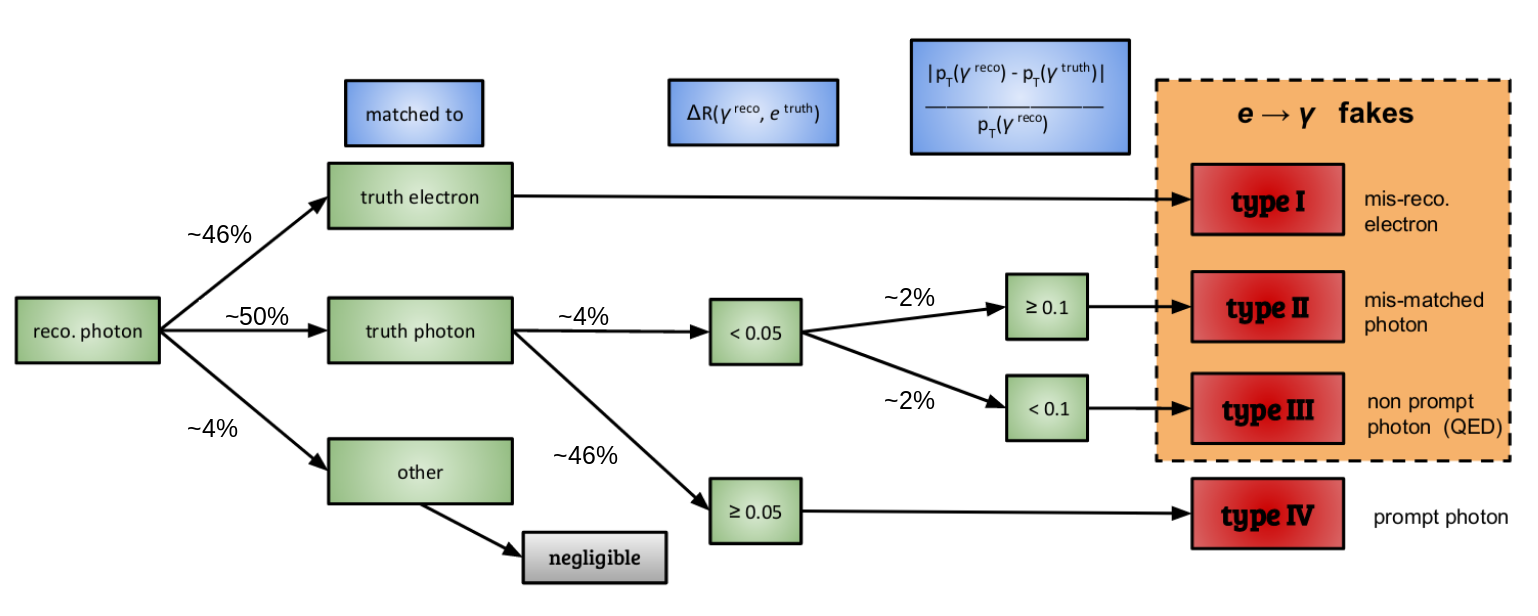
\includegraphics[width=\textwidth]{../../Thesis/ThesisImages/TruthStudyFakes.png}
\end{center}
Catagories: Simple mis-match, mis-match to truth photon (Reco pt $\geq$10\% higher than truth), non prompt photon, prompt photons
}

\subsection{Basic 1D Fake Rate Scale Factor}

\frame{Data and MC \frametitle{$m_{ee}, m_{e\gamma}$}
\begin{columns}
\begin{column}{0.02\textwidth}
\rotatebox{90}{$m_{e\gamma}$ \qquad \qquad \qquad $m_{ee}$\qquad} 
%\rotatebox{90}{Muon Channel        } 
\end{column}
\begin{column}{0.48\textwidth}
\begin{itemize}
\item Data
%\item  MCee integral small range: 424,051.  - Vgam: 429789 - All 430225
%\item DATAee integral small range: 468,832
%\item MCeg integral small range: 110822     - Vgam: 115066 - All 152420
%\item DATAeg integral small range: 118198
\end{itemize}
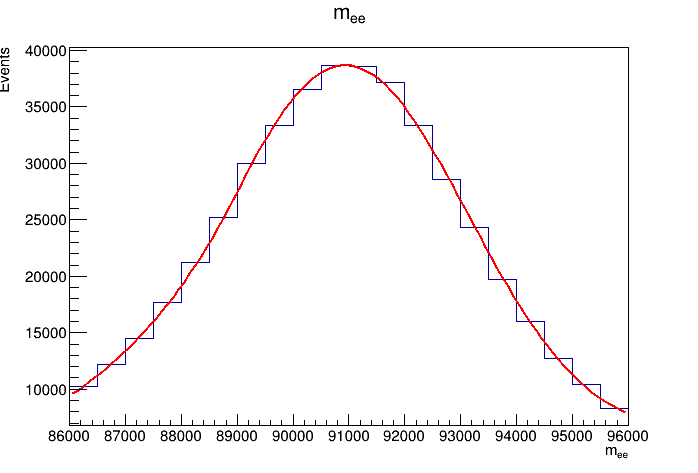
\includegraphics[width=.85\textwidth]{Images/Dataee.png} \\
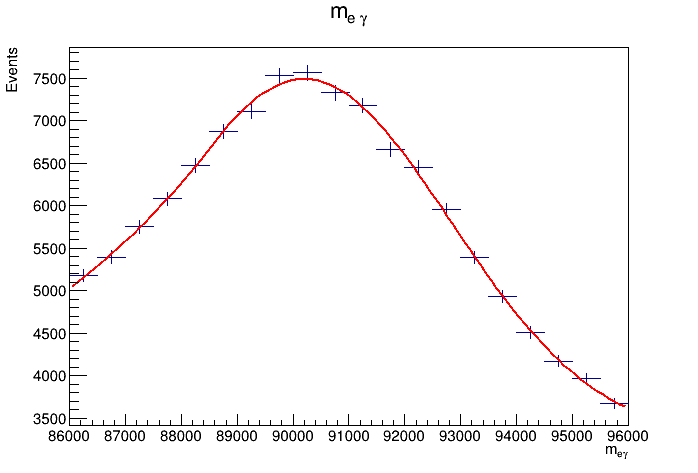
\includegraphics[width=.85\textwidth]{Images/Dataeg.png}
\end{column}
\begin{column}{0.48\textwidth}
\begin{itemize}
\item Monte Carlo
\end{itemize}
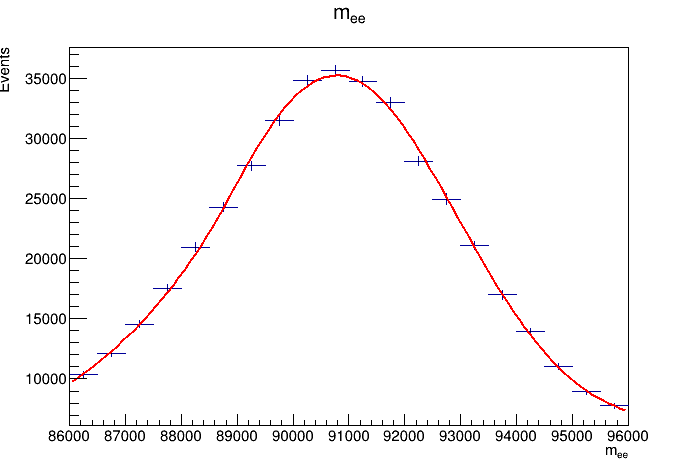
\includegraphics[width=.85\textwidth]{Images/MCVgamee.png} \\
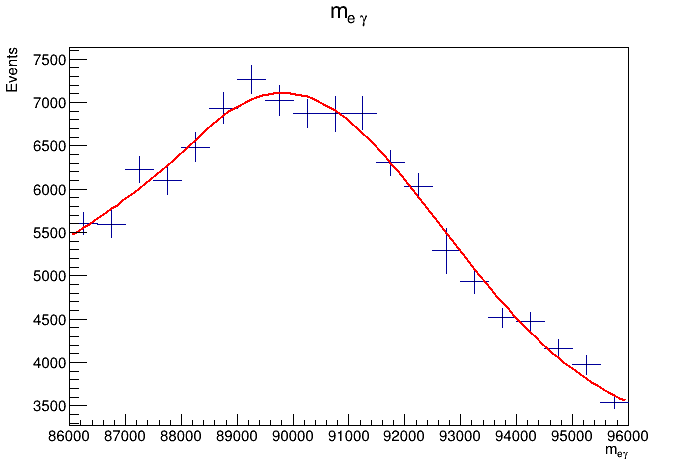
\includegraphics[width=.85\textwidth]{Images/MCVgameg.png}
\end{column}
\end{columns}
}


\frame{\frametitle{Scale Factor}
\[ \text{FR}^{\text{e-fake}}=\frac{N_{e,\gamma}}{N_{e,e}+N_{e,\gamma}}\]

\[  \text{SF}^{\text{e-fake}}_{\text{FR}} = \frac{\text{FR}^{\text{e-fake}}_{\text{data}}}{\text{FR}^{\text{e-fake}}_{\text{MC}}}\]
Basic Scale Factor can be calculated for the entire spectrum:
$\text{FR}^{\text{e-fake}}_{\text{data}} = 0.201$\\
$\text{FR}^{\text{e-fake}}_{\text{MC}} = 0.212$\\
$\text{SF}^{\text{e-fake}}_{\text{FR}} =0.953$
}

\frame{\frametitle{Scale Factors As Functions of Probe pt and eta}
\begin{columns}
\begin{column}{0.48\textwidth}
Probe $p_T$
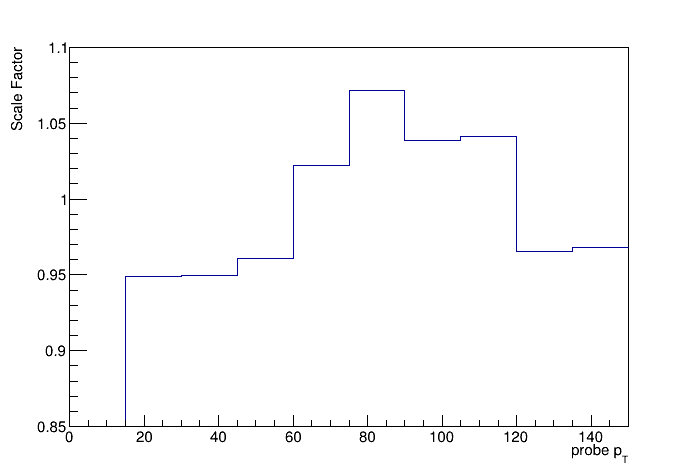
\includegraphics[width=\textwidth]{Images/pt1DSF.png}
\end{column}
\begin{column}{0.48\textwidth}
Probe $\eta$
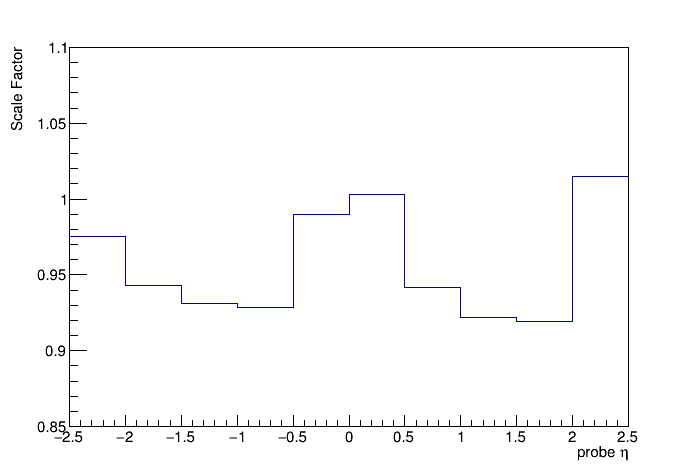
\includegraphics[width=\textwidth]{Images/eta1DSF.png}
\end{column}
\end{columns}
Good to check but in practice these are done using 2D Scale Factors
}

\subsection{2D Fake Rate Scale Factor}

\frame{\frametitle{Data and MC Distributions}
\begin{columns}
\begin{column}{0.02\textwidth}
\rotatebox{90}{ee region \qquad \qquad e$\gamma$ region\qquad} 
%\rotatebox{90}{Muon Channel        } 
\end{column}
\begin{column}{0.48\textwidth}
\begin{itemize}
\item Data
\end{itemize}
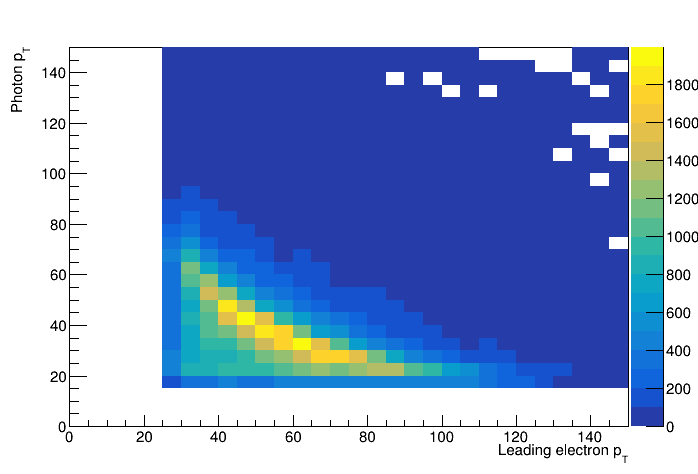
\includegraphics[width=.85\textwidth]{Images/dataPhotonElectronPT.png} \\
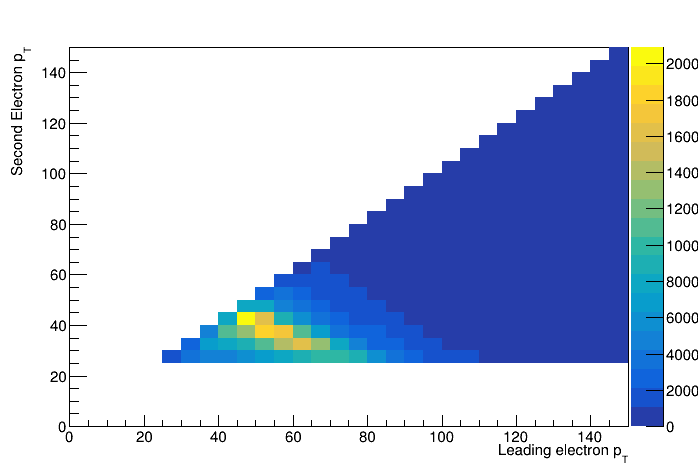
\includegraphics[width=.85\textwidth]{Images/dataElectronElectronPT.png}
\end{column}
\begin{column}{0.48\textwidth}
\begin{itemize}
\item Monte Carlo
\end{itemize}
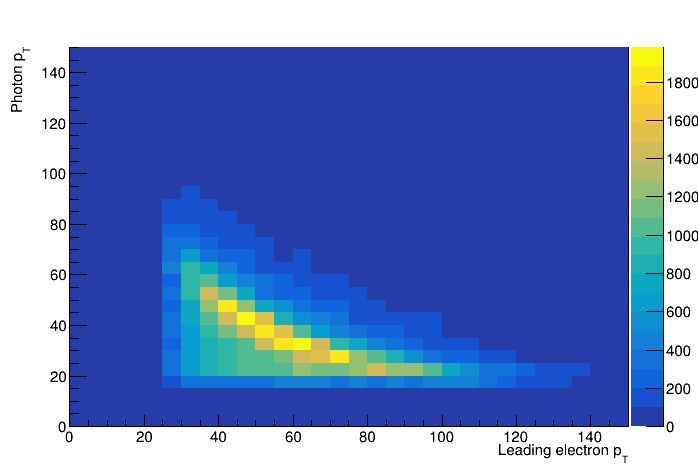
\includegraphics[width=.85\textwidth]{Images/mcPhotonElectronPT.png} \\
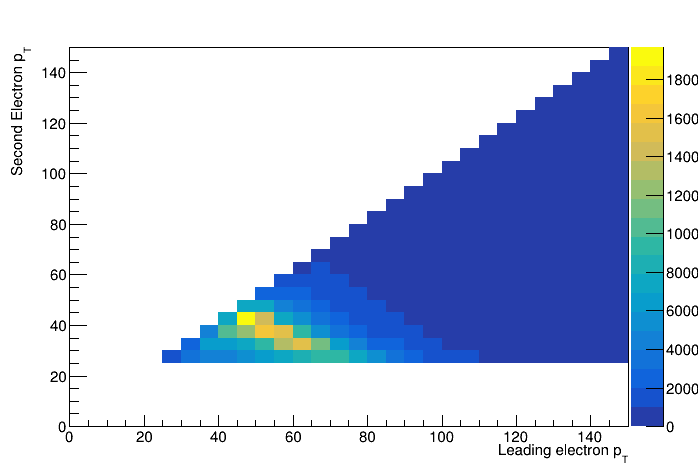
\includegraphics[width=.85\textwidth]{Images/mcElectronElectronPT.png}
\end{column}
\end{columns}
}

\frame{\frametitle{Next Steps - 2D Fake Rate}
\centering
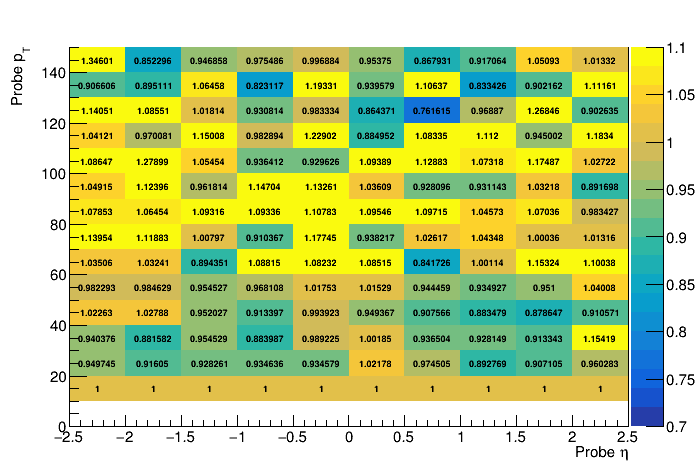
\includegraphics[width=\textwidth]{Images/2DSF.png}
}



%%%%%%%%%%%%%%%%%%%%%%%%%%%%%%%%%%%%%%%%%%%%%%%%%%%%%%%%%%%%%%%%%%
\section{Outlook and Conclusions}

\frame{\frametitle{Outlook}
\begin{itemize}
\item As always, still lots to be done
\item Fake Rate: $e\rightarrow\gamma$ has been investigated, further systematic investigations will continue
\item Fake Rate: $j\rightarrow \gamma$ to be investigated soon
\item Was able to squeak an extra factor of 2 out of Neural Network since I had to redo it for working points anyway
\item Questions?
\end{itemize}
}



%%%%%%%%%%%%%%%%%%%%%%%%%%%%%%%%%%%%%%%%%%%%%%%%%%%%%%%%%%%%%%%%

\appendix
\section{Backup}
\frame{\frametitle{Backup}
}
\frame{\frametitle{FCNC Diagrams}
\centering
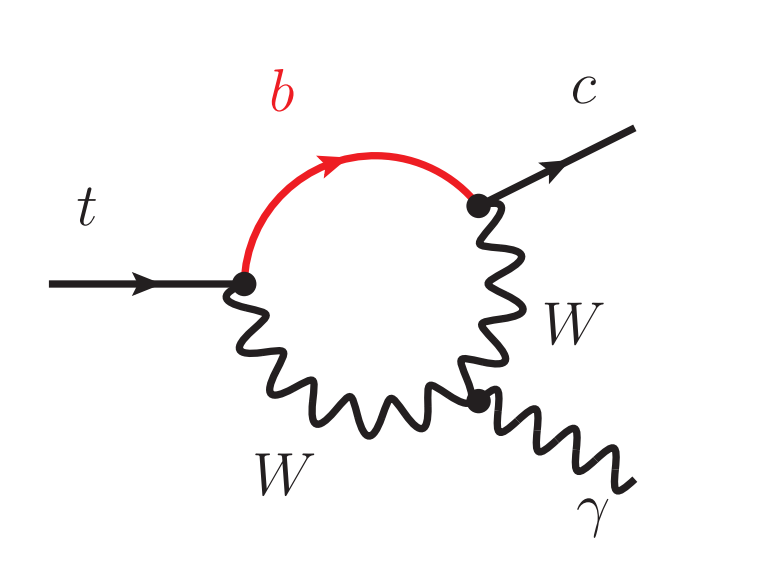
\includegraphics[width=.4\textwidth]{../../Thesis/ThesisImages/Theory/FCNCLoop.png}
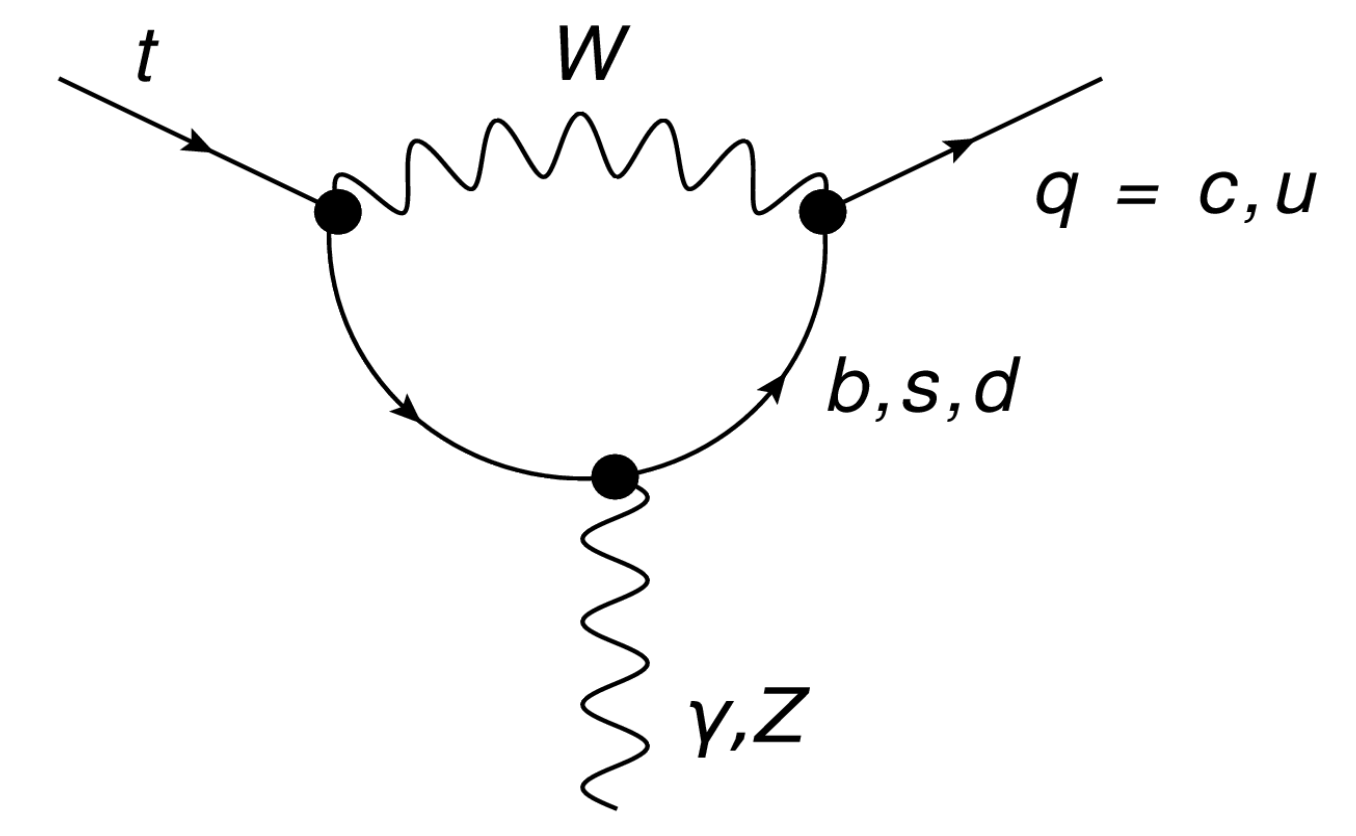
\includegraphics[width=.4\textwidth]{../../Thesis/ThesisImages/penguinFCNC.png}
}

\frame{\frametitle{NN Input Variable Correlations}
\centering
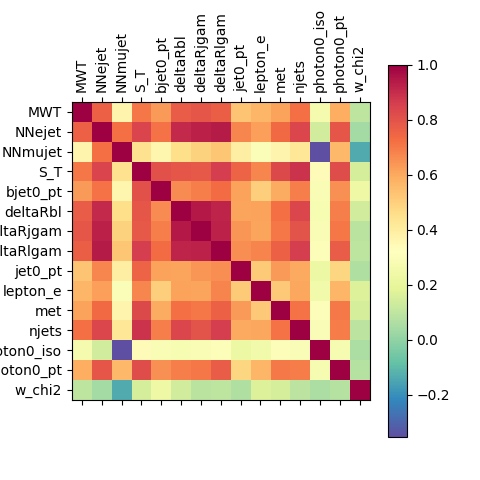
\includegraphics[height=.8\textheight]{Images/correlations.png}
}

\frame{\frametitle{Neural Network Model Inputs}
\centering
\scalebox{0.8}{ $\text{Separation} = \sum_{i}^{bins} \frac {n_{s i}-n_{b i}}{n_{s i}+n_{b i}}$}
\begin{columns}
\begin{column}{0.48\textwidth}
\centering
mu+jets channel\\
\scalebox{0.6}{\begin{tabular}{cc}
Variable & Separation \\
\hline
photon0iso & 41.18 \\
mqgam & 28.27 \\
photon0pt & 24.07 \\
mtSM & 11.60 \\
mlgam & 7.56 \\
deltaRjgam & 5.64 \\
deltaRbl & 4.42 \\
MWT & 3.34 \\
ST & 3.30 \\
nuchi2 & 3.12 \\
jet0pt & 2.81 \\
njets & 2.07 \\
smchi2 & 1.89 \\
wchi2 & 1.87 \\
jet0e & 1.52 \\
deltaRlgam & 1.17 \\
leptone & 0.87 \\
deltaRjb & 0.86 \\
met & 0.68 \\
bjet0pt & 0.52 \\
leptoniso & 0.27 \\
\end{tabular}
}
\end{column}
\begin{column}{0.48\textwidth}
\centering
e+jets channel \\
\scalebox{0.6}{\begin{tabular}{c c}
Variable & Separation\\
\hline
photon0pt & 23.14 \\
mqgam & 22.73 \\
photon0iso & 18.70 \\
mtSM & 11.02 \\
mlgam & 9.53 \\
deltaRbl & 5.00 \\
deltaRjgam & 4.60 \\
ST & 3.83 \\
MWT & 3.16 \\
jet0pt & 2.47 \\
njets & 1.70 \\
nuchi2 & 1.59 \\
deltaRlgam & 1.40 \\
wchi2 & 1.33 \\
smchi2 & 1.09 \\
deltaRjb & 0.88 \\
leptone & 0.85 \\
leptoniso & 0.56 \\
bjet0pt & 0.50 \\
met & 0.47 \\
\end{tabular}
}
\end{column}
\end{columns}
}

\frame{\frametitle{Input Variables}
['photon0iso','photon0pt','mqgam','mlgam','mtSM','deltaRjgam','deltaRbl',\\
'MWT','ST','njets','wchi2','jet0pt','deltaRlgam','leptone','met','bjet0pt']


}

\frame{\frametitle{Integrated Luminosity}
\centering
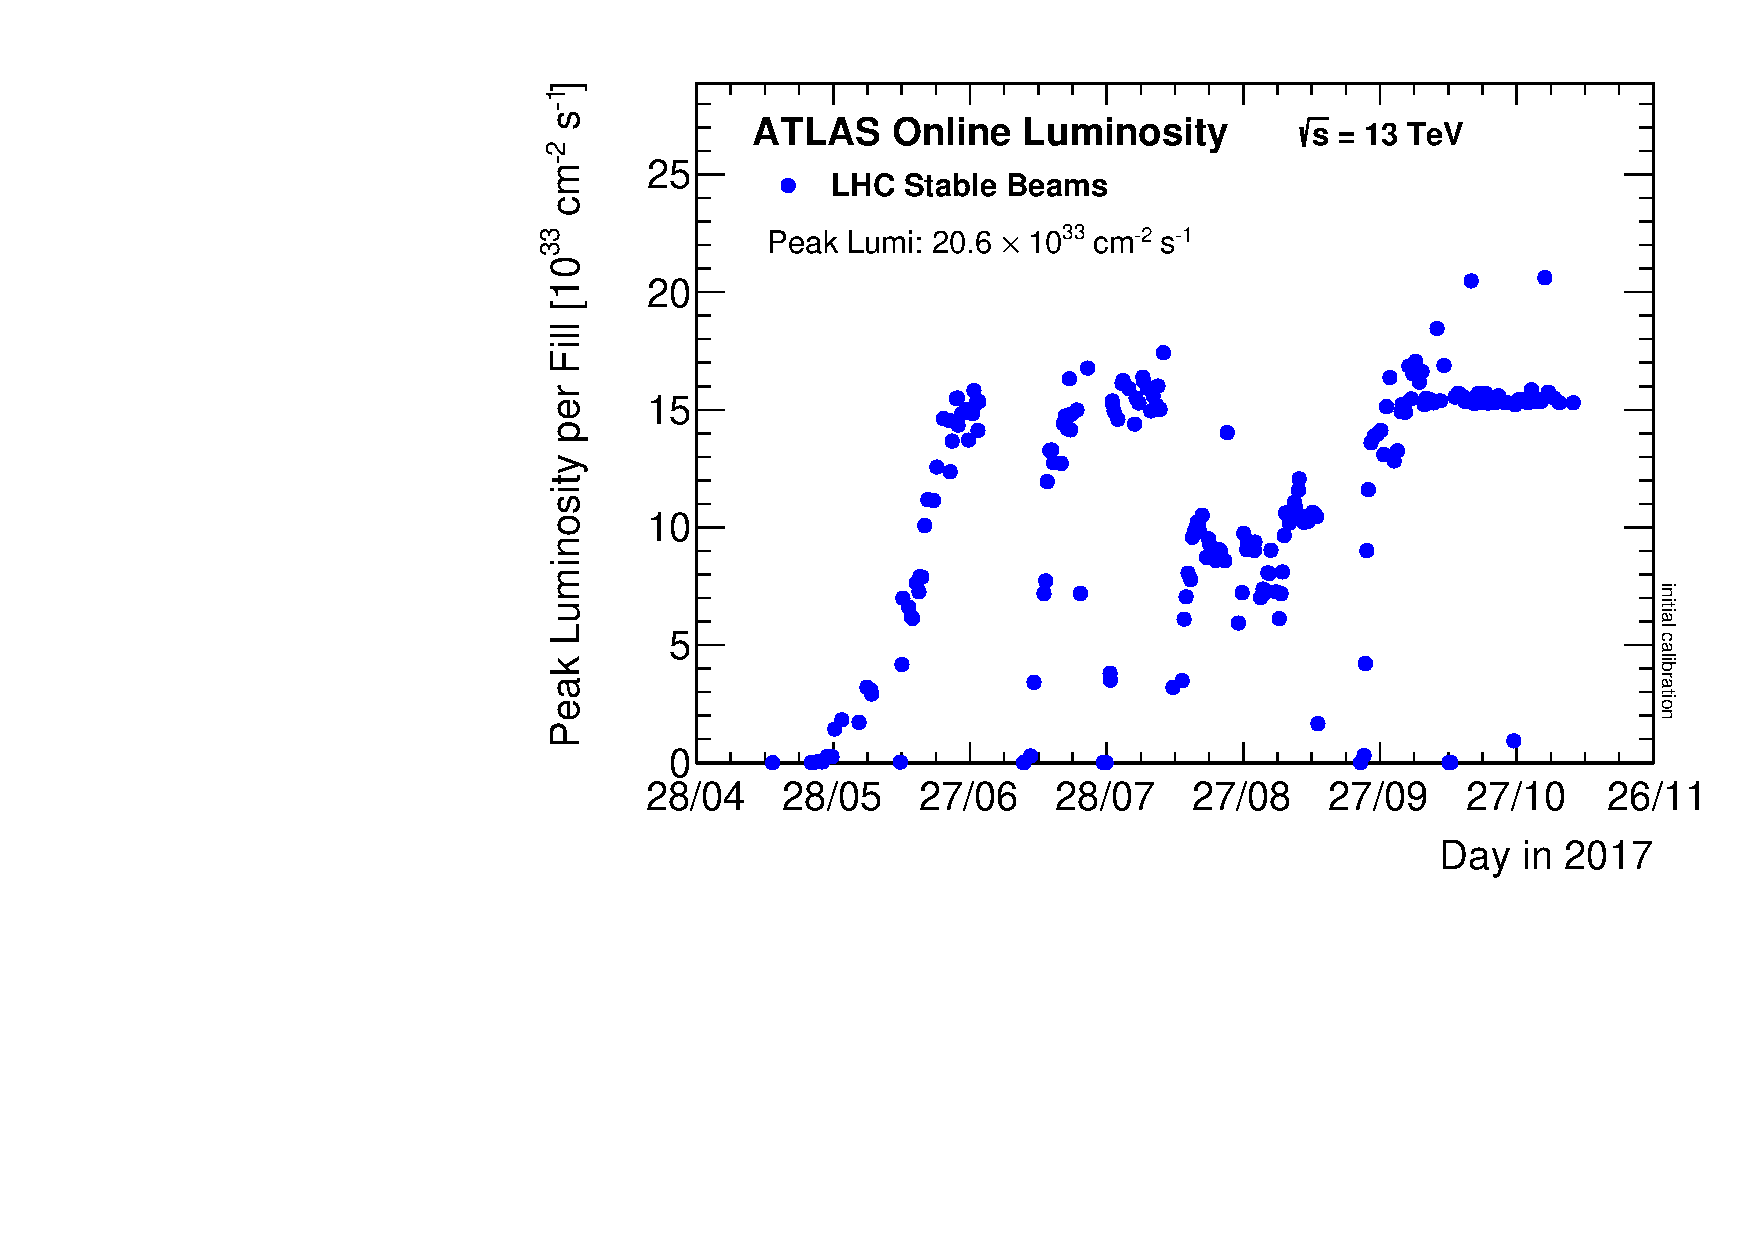
\includegraphics[width=1.\textwidth]{../../Thesis/ThesisImages/2017PeakLumiByFill.pdf}
}
\frame{\frametitle{A Couple BSM Diagrams}
\centering
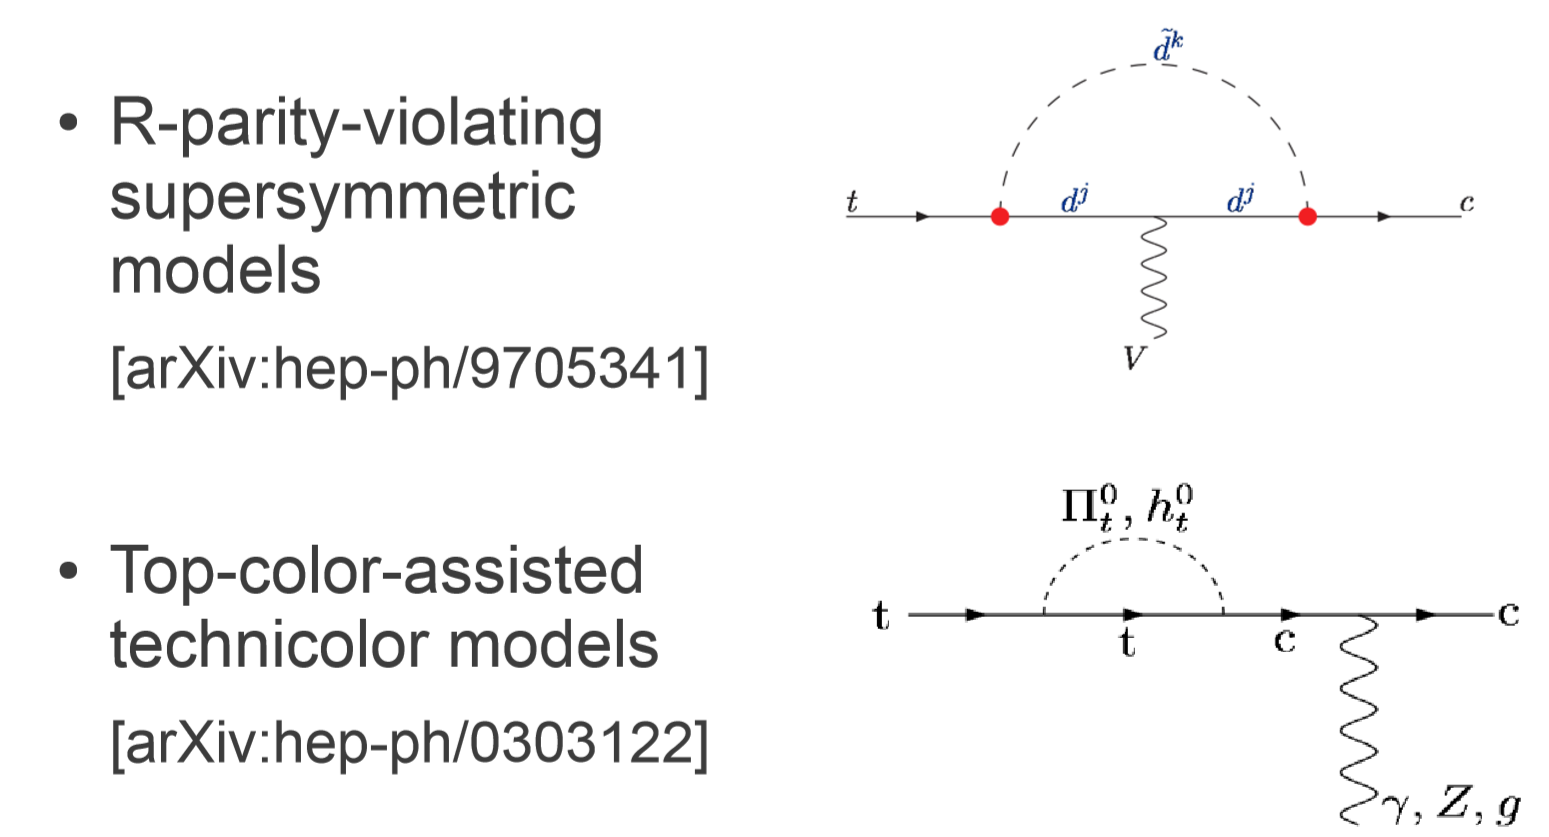
\includegraphics[width=1.\textwidth]{../../Thesis/ThesisImages/BSMDiagrams.png}
}

\frame{\frametitle{Jets/AntiKT}

\[ d_{ij} = min(\frac{1}{p_{ti}^2},\frac{1}{p_{tj}^2}) \frac{\Delta_{ij}^2}{R^2}
\]
\[ d_{iB} = \frac{1}{p_{ti}^2}
\]
\[ \Delta_{ij}^2 = (\eta_i -\eta_j )^2 + (\phi_i - \phi_j )^2
\]
\begin{itemize}
\item Find minimum of entire set of $\{ d_{ij},d_{iB} \}$
\item If $d_{ij}$ is the minimum particles i,j are combined into one particle and removed from the list of particles
\item If $d_{iB}$ is the minimum i is labelled as a final jet and removed from the list of particles
\item Repeat until all particles are part of a jet with distance between jet axes $\Delta_{ij}$ is greater than R
\end{itemize}
}

%\frame{\frametitle{B-tagging}
%\centering
%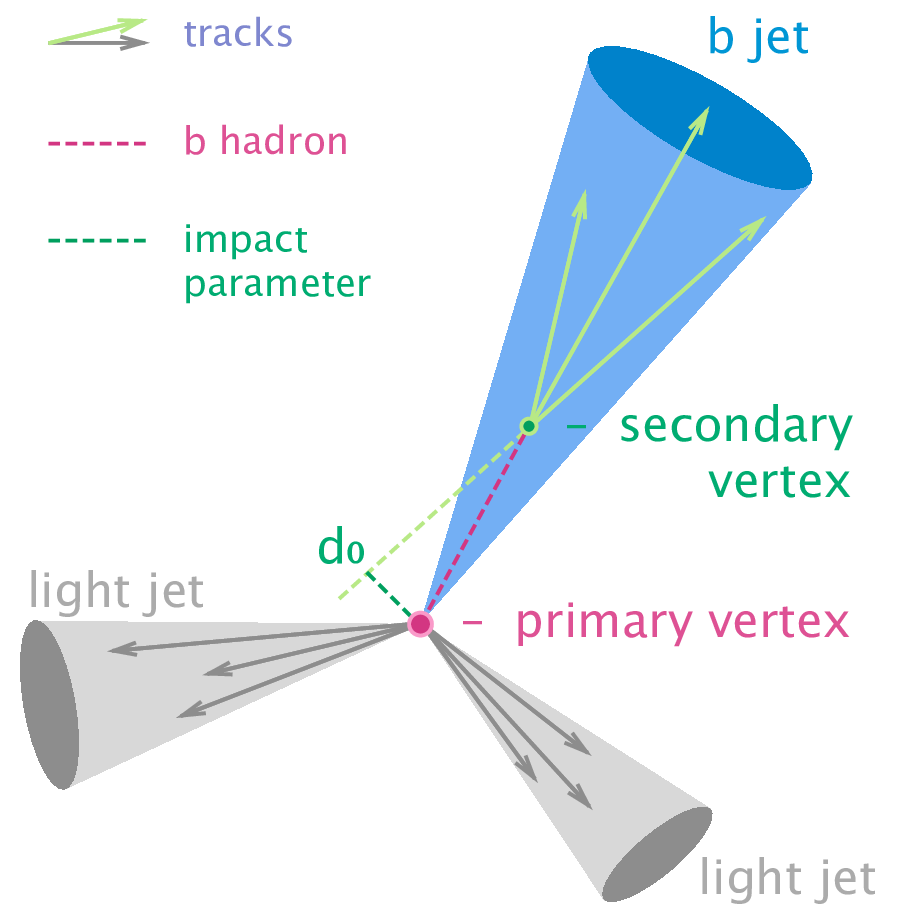
\includegraphics[height=.8\textheight]{../../Thesis/ThesisImages/SimulationNN/B-tagging_diagram.png}
%}

\frame{\frametitle{}
\[ \mathcal{L}^{eff}_{tq\gamma} = - e \bar{c} \frac{i \sigma^{\mu\nu}q_{\nu}}{m_t}(\lambda^{L}_{ct}P_L + \lambda^{R}_{ct}P_{R}) t A_{\mu} +H.c.
\]
}

\end{document}

%36.070


%%% Neural Net Ref: http://cs231n.github.io/neural-networks-1/

% npart0=['photon0_iso','photon0_pt','m_qgam','m_lgam','m_tSM','deltaRjgam','deltaRbl','MWT','S_T','nbjets','njets','w_chi2','jet0_pt','nu_chi2','sm_chi2','deltaRlgam','lepton_e','met','lepton_iso','bjet0_pt']
%all vars

%npart = ['photon0_iso','photon0_pt','m_qgam','m_lgam','m_tSM','deltaRjgam','deltaRbl','MWT','S_T','njets','nbjets','w_chi2','jet0_pt','deltaRlgam','lepton_e','met','bjet0_pt']
%usual npart1

%npart1=['photon0_iso','photon0_pt','deltaRjgam','deltaRbl','MWT','S_T','njets','w_chi2','jet0_pt','deltaRlgam','lepton_e','met','bjet0_pt']
%minimal